\chapter{Stokes Equations}\label{chap:stokes}

In this chapter we review the Stokes equations, the governing equations for low Reynolds number flow. These equations are appropriate for particulate flows, since the small length scales, the slow velocity, and the high viscosity of the solvent means that the Reynolds number is small. Using the Stokes equations instead of the more general Navier-Stokes equations provides significant simplifications. The Stokes equations do not contain a nonlinear inertial term, hence the fluid velocity can be written in terms of the boundary data when there are no non-conservative forcing terms. One of the  benefits of formulating the Stokes equations as a boundary integral equation is that it reduces the two-dimensional problem to a one-dimensional boundary integral. This leads to a method that naturally resolves complicated moving boundaries.

We will be modeling mobile rigid bodies suspended in a Stokesian fluid. These bodies interact hydrodynamically with each other and with solid walls. The suspended bodies will be rigid, meaning that they cannot change shape; they can only translate and rotate. This allows us to describe the position of a rigid body using only its center and an orientation angle. Its velocity can likewise be specified by a translational and a rotational velocity. 

\section{Fluid Equations}

We are interested in modeling  suspensions of rigid bodies, and this requires a good description of the state of the solvent. Given a domain $V\subset \mathbb{R}^2$ with boundary $S$, the state of a fluid can be described by the incompressible Navier-Stokes equations,
\begin{subequations}\label{eq:navier-stokes}
\begin{alignat}{2}
	\frac{\partial \uu}{\partial t} + \uu\cdot\nabla\uu  &= -\frac{1}{\rho}\nabla p + \nu\Delta\uu + \ff,\qquad&&\xx\in V,~t \geq 0, \label{eq:momentum_ns}\\
	\nabla\cdot\uu &= 0,\qquad&&\xx\in V,~t \geq 0,\label{eq:mass_ns}
\end{alignat}
\end{subequations}
where $\rho$ is the (constant) density, $p$ is the pressure, $\uu$ is the velocity, $\nu$ is the kinematic viscosity, and $\ff$ is an external body force acting on the fluid. Equation \eqref{eq:momentum_ns} is a statement of the conservation of momentum, and \eqref{eq:mass_ns}, the incompressibility condition, is a statement of conservation of mass. To close the formulation, boundary conditions and an initial condition for $\uu$ are required. We consider Dirichlet boundary conditions, along with an arbitrary initial condition
\begin{alignat*}{2}
	 \uu(\xx,t) &= \mathbf{g}(\xx,t), \qquad &&\xx\in S, t\geq 0\\
	  \uu(\xx,0) &= \uu_0(\xx), \qquad &&\xx\in V.
\end{alignat*}
To satisfy global conservation of mass, the boundary condition $\mathbf{g}$ must satisfy the no-flux compatibility condition
\[ \int_S \mathbf{g}\cdot\nn~\text{d}S = 0,\]
where $\nn$ is the unit normal on $S$. Since we are restricting ourselves to planar flows, the velocity $\uu$ is a vector in $\mathbb{R}^2$. 

Following well-established techniques for non-dimensionalization, we pick a characteristic length scale $\ell$, a characteristic velocity scale $U$, a characteristic time scale $\tau$, and make the following substitutions:
\begin{equation}\label{eq:dimensions} \xx^* = \xx/\ell, \qquad \uu^* = \uu/U,\qquad t^* = t/\tau, \qquad p^* = p\ell/(\rho\nu U),\qquad \ff^* =\ff/|\ff|. \end{equation}
This leads to the non-dimensionalized Navier-Stokes equations,
\begin{align*} St\frac{\partial\uu^*}{\partial t^*} + \uu^*\cdot\nabla^*\uu^* &= - \frac{1}{Re}\nabla^* p^* + \frac{1}{Re}\Delta^*\uu^* + \frac{1}{Fr^2}\ff^*,\\
	\nabla\cdot\uu^* &= 0,\end{align*}
where $St = \ell/(U\tau)$ is the Strouhal number, $Fr = U/\sqrt{\ell|\ff|}$ is the Froude number, and $Re= \ell U/\nu$ is the Reynolds number. If $Re \ll1$ and $St \ll1/Re$ then the terms with $1/Re$ dominate and the remaining terms can be neglected. This gives the nondimensional steady incompressible Stokes equations,
\begin{subequations}\label{eq:stokes}
\begin{alignat}{2}
	-\Delta \uu + \nabla p &= \frac{1}{Fr^2}\ff,\qquad&& \xx\in V,\label{eq:stokes_mom}\\
	\nabla\cdot\uu &= 0,\qquad&& \xx\in V,\\
	\uu &= \uu_b,\qquad &&\xx\in S.
\end{alignat}
\end{subequations}
For notational clarity we have dropped the asterisk superscript, however, $\uu$, $p$, $\ff$, and all the derivatives are non-dimensionalized according to \eqref{eq:dimensions}. For the remainder of this dissertation, whenever we speak of the Stokes equations, we mean the incompressible, steady, nondimensional, Stokes equations \eqref{eq:stokes}. The Stokes equations are the governing equations for small scale, slow moving, viscous flows. These are precisely the kind of flows encountered in most particulate flows. 

Defining the stress tensor $\bm{\sigma}$ to be
\[\ssigma = -p\mathbf{I}+ \frac{1}{2}\left(\nabla \uu + (\nabla\uu)^T\right),\]
the momentum balance \eqref{eq:stokes_mom} can be written as
\[ \nabla \cdot\bm{\sigma} =\frac{1}{Fr}\ff,\qquad \xx\in V.\]
The stress tensor has a static contribution from the pressure and a dynamic contribution from viscous forces and is often written as,
\begin{equation*}\label{eq:stress} 
 \ssigma = -p\mathbf{I}+\ee,
 \end{equation*}
where $\ee = (\nabla\uu + (\nabla\uu)^T)/2$ is the strain rate tensor and represents the contribution of viscous forces to the total stress.

In many practical cases, $\ff$ is a conservative field and can therefore be expressed as the gradient of a scalar field and included in the pressure gradient, thus leaving a homogeneous equation. In this case, the momentum balance for the Stokes equations is
\[ \nabla\cdot\ssigma = 0, \qquad \xx \in V.\]

The Stokes equations represent a significant simplification of the Navier-Stokes equations. By neglecting the nonlinear $\uu\cdot\nabla\uu$ term and the time dependent $\partial\uu/\partial t$ term, we obtain a set of linear, time-independent, elliptic equations. Because of the linearity, the superposition principle applies. This makes the Stokes equations much easier to analyze mathematically than the Navier-Stokes equations. For example, it is known that given appropriate boundary conditions, a solution to the three-dimensional Stokes equations exists and is unique (up to a constant for the pressure). By contrast, existence and uniqueness of the three-dimensional incompressible Navier-Stokes equations is an unresolved problem, and is one of the Millennium Prize problems \cite{Carlson2006}.

\section{Rigid Body Motion}

This dissertation is concerned with rigid (i.e. non-deforming) bodies. When such a body moves, it must do so without changing shape, meaning that it can only translate and rotate. For a body in $\mathbb{R}^3$ with a center of rotation $\cc$, all rigid body motions can be expressed as
\begin{equation}\label{eq:rbm}\uu^{\text{RBM}}(\xx) = \UU + \bm{\omega}\times(\xx - \cc),\end{equation}
where $\UU\in\mathbb{R}^3$ is a constant translational velocity and $\bm{\omega}\in\mathbb{R}^3$ is a constant angular velocity. In $\mathbb{R}^2$, $\bm{\omega} = (0, 0, \omega)$, so a rigid body motion is 
\[ \uu^{\text{RBM}} = \UU + \omega(\xx - \cc)^\perp,\]
where $\xx^\perp = \langle -x_2, x_1\rangle$. Once we know the translational and rotational velocities of a body undergoing a rigid body motion, equation \eqref{eq:rbm} gives the velocity at any point inside that body. 

Proposition \ref{prop:stress} shows that the stress field associated with rigid body motion is zero everywhere. The associated proof uses the standard third-order Levi-Civita tensor to denote the cross product in $\mathbb{R}^3$, however the result holds in $\mathbb{R}^2$, where $\omega_1 = \omega_2 = 0$. 

\begin{proposition}
\label{prop:stress}
The stress tensor of a rigid body motion is zero. 
\end{proposition}
\begin{proof}
Twice the strain rate $2\ee = (\nabla\uu^{\text{RBM}} + (\nabla\uu^{\text{RBM}})^T)$ of a rigid body motion satisfies
\begin{align*}
	 2e_{ij} &= \partial_i\left(U_j + \epsilon_{jk\ell} \omega_k (x_\ell - c_\ell)\right) + \partial_j\left(U_j + \epsilon_{ik\ell}\omega_k (x_\ell - c_\ell)\right)\\
	 &= \epsilon_{jk\ell}\partial_i\left(\omega_k(x_\ell - c_\ell)\right) + \epsilon_{ik\ell}\partial_j\left(\omega_k(x_\ell - c_\ell)\right)\\
	 &=\epsilon_{jk\ell}\omega_k\delta_{i\ell} + \epsilon_{ikl}\omega_k\delta_{j\ell}\\
	 &= \epsilon_{jki}\omega_k + \epsilon_{ikj}\omega_k.
 \end{align*}
 Since, by definition, $\epsilon_{jki} = -\epsilon_{ikj}$, it follows that $e_{ij} = 0$.
 
By equation \eqref{eq:stokes_mom},  $\Delta \uu^{\text{RBM}} = \nabla p$. Since $\uu^{\text{RBM}}$ is linear in $\xx$, $\Delta \uu^{\text{RBM}} = \nabla p = 0$. Thus, the pressure of a rigid body motion is constant, and typically is taken to be zero. Therefore, the total stress of a rigid body motion, $\bm{\sigma} = -p\mathbf{I} + \ee$, is zero.
\end{proof}

Each rigid body is subject to a net force and torque. For a rigid body with boundary $S$, unit normal $\nn$, and center of rotation $\cc$, the hydrodynamic component of the force and torque $\FF$ and $L$, respectively, are
\[ \FF = \int_S \ff ~\text{d}S, \qquad L = \int_S (\xx-\cc)^\perp \cdot\ff~\text{d}S,\]
where $\ff = \bm{\sigma}\cdot\nn$ is the fluid traction acting on the body. In order to study how rigid bodies move under the influence of forces and torques, we need to solve the equations of motion,
\begin{equation}\label{eq:motion} m \frac{d \UU}{d t} = \FF, \qquad  I \frac{d \omega}{dt} = L,\end{equation}
where $m$ is the mass of the body and $I$ is its rotational inertia. Assuming the body has a constant density $\rho$, then $I = \rho\int_A |\xx - \cc|^2~\text{d}A$, where $A$ is the cross-sectional area of the particle. Scaling time in \eqref{eq:motion} by $\ell/U$ and the force by $\nu U \ell/\rho$ we have
\[ Re \frac{m}{\rho \ell^3}\frac{d \UU}{dt} = \FF, \qquad Re \frac{I}{\rho\ell^5}\frac{d\omega}{dt} = L.\]
Thus when $\Re \ll 1$,  the bodies undergo no acceleration. This is the basis for the \emph{quasistatic} approximation. The fact that the bodies are not accelerating means that \eqref{eq:motion} is not needed, and that the body center $\cc$ and angle $\theta$  evolve according to
\[ \frac{d \cc}{dt} = \UU,\qquad \frac{d\theta}{dt} = \omega.\]
The quasistatic approximation allows us to solve a sequence of steady Stokes equations, even as the rigid bodies move and the geometry changes. The fluid is assumed to instantaneously adjust to the new geometry.


\section{Integral Representation}\label{sec:bie}

In the homogeneous case (when $\ff$ is conservative), potential theory and Green's identity allow us to represent the solution to the Stokes equations as an integral of the fluid velocity and traction on $S$. This leads to a dimension reduction, and once we know the velocity and traction on the boundary, the solution at any point inside $V$ is represented as a boundary integral. The major advantage of this dimension reduction is that it simplifies discretizing complicated geometries. 

The first step to develop an integral equation formulation is to compute the fundamental solution of \eqref{eq:stokes}. This is a pair of functions $\uu(\xx)$ and $p(\xx)$ satisfying
\begin{subequations}\label{eq:fundamental}
\begin{alignat}{2}
	\nabla \cdot \sigma = \Delta\uu - \nabla p &= -\FF\delta(\xx-\xx_0),\qquad&&\xx\in \mathbb{R}^2,\label{eq:fundamental_mom}\\
	\nabla\cdot\uu &= 0,\qquad&&\xx\in\mathbb{R}^2,
\end{alignat}
\end{subequations}
where $\delta(\xx-\xx_0)$ is the Dirac delta function centered at $\xx_0$. We note that the choice of sign on the right hand side of \eqref{eq:fundamental_mom} is arbitrary and an equivalent formulation exists if a positive sign is used. A detailed discussion of distributions, including the Dirac delta function, is found in many textbooks, e.g. \cite{Griffel2002}. For our purposes, however, \eqref{eq:fundamental_mom} means that:
\begin{enumerate}
	\item $\nabla\cdot\ssigma = 0$ for all $\xx \ne \xx_0$,
	\item $\int_{\mathbb{R}^2} \nabla\cdot\ssigma~\text{d}V = -\FF$. 
\end{enumerate}

In $\mathbb{R}^2$ 
\begin{align*}
	\uu(\xx) = \frac{\FF\cdot \mathcal{G}(\xx,\xx_0)}{4\pi}, \qquad p(\xx) = \frac{\FF\cdot\mathcal{P}(\xx,\xx_0)}{4\pi},
\end{align*}
satisfies \eqref{eq:fundamental} \cite{Pozrikidis1992}, where
\[ \mathcal{G}_{ij}(\xx,\xx_0) = -\delta_{ij}\ln r + \frac{r_i r_j}{r^2}, \qquad \mathcal{P}_j(\xx,\xx_0) = \frac{2 r_j}{r^2} + P_j^\infty,\]
and $\rr = \xx - \xx_0$, $r = |\rr|$, $\mathcal{G}(\xx,\xx_0)$ is called the Oseen tensor, and $\mathcal{G}(\xx,\xx_0)/(4\pi)$ is called the Green's dyadic. The pressure only appears as a gradient in the Stokes equations and is therefore only determined up to the constant $P_j^\infty$.  By combining the velocity and the pressure, the corresponding stress tensor is
\[ \sigma_{ij}(\xx) = \frac{T_{ijk}(\xx,\xx_0)F_k}{4\pi} ,\]
where
\[ T_{ijk}(\xx,\xx_0) = -4\frac{r_i r_j r_k}{r^4}.\]

The solution of any eliptic homogeneous PDE can be represented in terms of integrals along the boundary of the domain of the solution and its derivatives. An example is Green's third identity for the Laplace equation. If $w(\mathbf{x})$ is a harmonic function, then 
\[ w(\mathbf{x}) = \int_S w(\yy)\frac{\partial}{\partial\nn}\left(\frac{1}{2\pi} \log | \xx -\yy |\right)~\text{d}s(\yy) - \frac{1}{2\pi}\int_S\log |\xx - \yy| \frac{\partial w}{\partial\nn}~\text{d}s(\yy).\]

 The solution to the Stokes equations can be written in terms of boundary integrals of $\uu$ and the surface traction $\ff = \ssigma\cdot\nn$, where $\nn$ is the unit normal pointing out of the fluid domain. By applying the Lorenz reciprocal theorem \cite{Karrila1991, Ladyzhenskaya1963,Pozrikidis1992}
\begin{equation}\label{eq:integral_form}\uu(\xx) = -\int_S  \frac{f_i(\yy)\mathcal{G}_{ij}(\xx , \yy)}{4\pi}~\text{d}S(\yy) + \int_S u_i(\yy) T_{ijk}(\xx , \yy)n_k(\yy)~\text{d}S(\yy),\qquad \xx\in V.\end{equation}
Equation \eqref{eq:integral_form} expresses $\uu(\xx)$ for $\xx\in V$ in terms of $\uu$ and $\ff$ on $S$. 

The first term in \eqref{eq:integral_form},
\begin{equation}\label{eq:slp_primative}
	\mathcal{S}[\ff](\xx) = \int_S  \frac{f_i(\yy)\mathcal{G}_{ij}(\xx , \yy)}{4\pi}~\text{d}S(\yy) ,
\end{equation}
is known as the \emph{single-layer potential}. This represents the velocity field generated by the force distribution $\ssigma(\yy)\cdot\nn(\yy)$ along $S$. The second term,
\begin{equation}\label{eq:dlp_primative}
 \mathcal{D}[\uu](\xx) = \int_S u_i(\yy) T_{ijk}(\xx , \yy)n_k(\yy)~\text{d}S(\yy),
\end{equation}
is known as the \emph{double-layer potential}. Thus \eqref{eq:integral_form} can be written as
\[ \uu(\xx) = -\mathcal{S}[\ff](\xx) + \mathcal{D}[\uu](\xx) ,\qquad \xx\in V.\]
We will on occasion write the single-layer and double-layer potentials as
\[ \mathcal{S}[\ff](\xx) = \int_S f_i(\yy) W_{ij}(\xx,\yy)~\text{d}S(\yy), \qquad \mathcal{D}[\uu](\xx) = \int_S u_i(\yy)K_{ij}(\xx,\yy)~\text{d}S(\yy),\]
where $\WW$ and $\KK$ are the kernels of the single- and double-layer potentials, respectively, given by
\begin{subequations}
	\begin{align}
		 W_{ij}(\xx,\yy) &= \frac{\mathcal{G}_{ij}(\xx,\yy)}{4\pi},\\ \qquad K_{ij}(\xx,\yy) &=T_{ijk}(\xx,\yy)n_k(\yy).\label{eq:dlp_kernel}
	\end{align}
\end{subequations}

The point $\yy\in S$ in the layer potentials is known as the source point and the point $\xx\in V\cup S$ is known as the target point. While equation \eqref{eq:integral_form} holds for any target point $\xx\in V$, it is false if $\xx\in S$. This is due to a jump in the double-layer potential. If we let $\xx\in S$ and assume the boundary has a continuous tangent vector, the double-layer potential satisfies the following conditions for $\xx\in S$:
\begin{subequations}\label{eq:jump_conditions}
\begin{alignat}{2}
	\mathcal{D}[\uu](\xx)_{(i)} &:=  \lim\limits_{\epsilon\to 0} \mathcal{D}[\uu](\xx - \epsilon \nn(\xx)) = -\frac{1}{2}\uu(\xx)+ \mathcal{D}[\uu](\xx)\label{eq:jump_interior},\\
	\mathcal{D}[\uu](\xx)_{(e)} &:=  \lim\limits_{\epsilon\to 0} \mathcal{D}[\uu](\xx +\epsilon \nn(\xx)) = +\frac{1}{2}\uu(\xx)+ \mathcal{D}[\uu](\xx).\label{eq:jump_exterior}
\end{alignat}
\end{subequations}
However, the single-layer potential does not have such a jump and satisfies:
\begin{alignat*}{2}
	\mathcal{S}[\ff](\xx)_{(i)} &:=  \lim\limits_{\epsilon\to 0} \mathcal{S}[\ff](\xx - \epsilon \nn(\xx)) =  \mathcal{S}[\ff](\xx),\\
	\mathcal{S}[\ff](\xx)_{(e)} &:=  \lim\limits_{\epsilon\to 0} \mathcal{S}[\ff](\xx +\epsilon \nn(\xx)) =  \mathcal{S}[\ff](\xx).
\end{alignat*}
Therefore, the jumps in the layer potentials at $\xx\in S$ are
\begin{align*}
	 \llbracket \mathcal{S}[\ff](\xx)\rrbracket &:= \mathcal{S}[\ff](\xx)_{(e)} - \mathcal{S}[\ff](\xx)_{(i)} = \mathbf{0},\\
	 \llbracket \mathcal{D}[\uu](\xx)\rrbracket &:= \mathcal{D}[\uu](\xx)_{(e)} - \mathcal{D}[\uu](\xx)_{(i)} = \uu(\xx).
\end{align*}
We note that the jump in the traction of the single-layer is $\ff$, and this is often used to balance the fluid force with the elastic force of deformable (non-rigid) bodies \cite{Rahimian2010, Quaife2014, Quaife2015}. In contrast, the traction of the double-layer is continuous through $S$. This fact is used in Proposition \ref{prop:net_force}. 

Letting $\xx\in S$ and using the jump condition  of the double-layer potential \eqref{eq:jump_interior}, we have the boundary integral equation (BIE)
\begin{equation}\label{eq:bie} \mathcal{S}[\ff](\xx) + \mathcal{D}[\uu](\xx) = \frac{1}{2}\uu(\xx),\qquad \xx\in S.\end{equation}
Assuming that we know the velocity on $S$, \eqref{eq:bie} allows us to compute the traction on $S$ and vice versa. Thus \eqref{eq:bie} is the Stokes analog of the Dirichlet to Neumann map for Laplace's equation. Solving \eqref{eq:bie} followed by applying \eqref{eq:integral_form} is known as a direct BIE formulation.

Instead of using $\uu$ to compute $\ff$ (or vice-versa) and then applying \eqref{eq:integral_form}, we use an indirect integral equation formulation. This is done by representing $\uu$ with an arbitrary, non-physical, density function of the single- or double-layer potentials. For example, we could represent $\uu$ as a single-layer potential with density $\bm{\zeta}(\xx)$, 
\begin{equation}\label{eq:slp_vol}\uu(\xx) = \mathcal{S}[\pmb{\zeta}](\xx), \qquad \xx \in V.\end{equation}
Recalling that $\llbracket\mathcal{S}[\bm{\zeta}](\xx)\rrbracket= \mathbf{0}$, and letting $\xx \to S$ gives the indirect BIE
\begin{equation}\label{eq:bie_slp}\mathcal{S}[\bm{\zeta}](\xx) = \mathbf{g}(\xx) \qquad \xx\in S.\end{equation}
That is, \eqref{eq:bie_slp} is solved for the density function $\bm{\zeta}(\xx)$ that guarantees the boundary condition $\uu(\xx) = \mathbf{g}(\xx)$, $\xx\in S$ is satisfied. Then $\uu(\xx)$ is evaluated for $\xx\in V$ with \eqref{eq:slp_vol}. Likewise, we could represent the velocity as a double-layer potential with an arbitrary function density $\bm{\eta}(\xx)$,
\begin{equation}\label{eq:dlp_vol}\uu(\xx) = \mathcal{D}[\bm{\eta}](\xx), \qquad \xx\in V.\end{equation}
Recalling that $\llbracket\mathcal{D}[\bm{\eta}](\xx)\rrbracket = \bm{\eta}(\xx)$ and letting $\xx \to S$ (from inside $V$) gives the indirect BIE
\begin{equation}\label{eq:bie_dlp} -\frac{1}{2}\bm{\eta}(\xx) + \mathcal{D}[\bm{\eta}](\xx) = \mathbf{g}(\xx), \qquad \xx\in S.\end{equation}
As in the single-layer equation \eqref{eq:bie_slp}, the density function $\bm{\eta}$ ensures that the boundary condition for $\uu$ is satisfied. We solve \eqref{eq:bie_dlp} for the density function $\bm{\eta}(\xx)$  and then use the density function in \eqref{eq:dlp_vol} to evaluate the $\uu(\xx)$ for $\xx\in V$. 

Regardless of whether we use a single-layer or double-layer ansatz for $\uu$ we must solve a BIE. The Fredholm alternative and spectral theorem allow us to analyze the solvability and stability of the BIEs \eqref{eq:bie_slp} and \eqref{eq:bie_dlp}. This is discussed in the following section.

\subsection{Fredholm Equations}\label{sec:fredholm}

A general Fredholm integral equation is
\begin{equation}\label{eq:fredholm} \lambda z(\xx) - \int_S K(\xx,\yy)z(\yy)~\text{d}S(\yy) = g(\xx), \qquad \xx\in S,\end{equation}
where $\lambda$ is a given constant, $g:S\to\mathbb{R}$ is continuous, and $K(\xx,\yy): S\times S\to \mathbb{R}$ is continuous and at worst weakly singular, i.e.,
\[\int_S\left( \int_{S}| K(\xx, \yy)|~\text{d}S(\yy)\right)~\text{d}S(\xx) < \infty.\]
Typically, the function $g(\xx)$ is a boundary condition, $K(\xx,\yy)$ is related to the fundamental solution of the PDE of interest, and $\lambda$ depends on the choice of $K$. We are interested in solving for $z: S \to\mathbb{R}$. If $\lambda = 0$, \eqref{eq:fredholm} is called a first-kind Fredholm integral equation, otherwise it is a second-kind Fredholm integral equation. Therefore, \eqref{eq:bie_slp} is a first-kind Fredholm integral equation and \eqref{eq:bie_dlp} is a second-kind Fredholm integral equation. Fredholm integral equations may be written in the abstract notation
\begin{equation}\label{eq:fredholm-abstract} \lambda z - \mathcal{K}z = g.\end{equation}
For example, the double-layer BIE \eqref{eq:bie_dlp} can be written in this form, with $\lambda = -1/2$ and $\mathcal{K} = -\mathcal{D}$.  

We now discuss the behavior and solvability of \eqref{eq:bie_slp} and \eqref{eq:bie_dlp}. To begin, some background on compact operators in necessary. The following follows closely to \cite{Karrila1991} where the discussion is framed in the context of BIEs; more details on compact operators can be found in standard texts on functional analysis, e.g.  \cite{Griffel2002}. Because  of the integrability of $K(\xx,\yy)$, $\mathcal{K}$ is a compact linear operator on $\text{L}^2(S)$. Therefore, by the spectral theorem, the eigenvalues of $\mathcal{K}$ cluster only at the origin, and it can be approximated to any precision with a finite rank linear operator (i.e. a matrix). This will play a fundamental role when we consider discretizations of BIEs in Chapter \ref{chap:numerics}.

Consider a compact operator on a Hilbert space $\text{H}$ ($\text{L}^2(S)$ is a Hilbert space). A compact operator is any operator that maps a bounded set to a relatively compact set. Every finite dimensional bounded set is relatively compact. Compact operators form a subset of bounded operators, meaning that every compact operator is necessarily bounded. It follows that identity operator $I$ is compact if and only if $H$ is finite dimensional, since in an infinite dimensional space, the identity maps bounded sets that are not relatively compact to themselves.  Multiplication by a bounded operator from either the left or the right preserves compactness. 

From this, we can deduce that an infinite dimensional compact operator $\mathcal{K}$ cannot have a bounded inverse. To show this, we observe that if $\mathcal{K}^{-1}$ is bounded, then $I = \mathcal{K}\mathcal{K}^{-1}$ must also be compact, since multiplication by a bounded operator preserves compactness. This contradicts the statement that the identity is not compact on infinite dimensional spaces. Therefore, the inverse of a first-kind Fredholm integral equation is unbounded, meaning that small changes in the data $g$ lead to arbitrarily large changes to the solution $z$. At a numerical level, the unboundedness results in a matrix with an increasing condition number as the discretization is refined. 

The inverse of a second-kind integral equation, however can be bounded. The Fredholm alternative states that either a second-kind Fredholm integral equation of the form \eqref{eq:fredholm-abstract} has a unique solution for any $g$, or the corresponding homogeneous equation
\[ \lambda z- \mathcal{K}z = 0\]
has nontrivial solutions. This is  analogous to the invertible matrix theorem of linear algebra. If the homogeneous equation has nontrivial solutions, then these solutions are null functions of \eqref{eq:fredholm-abstract} and also eigenfunctions of the operator $\mathcal{K}$ corresponding to the eigenvalue $\lambda$, since the null functions satisfy
\[ \mathcal{K}z = \lambda z.\]
If $\lambda$ is not an eigenvalue of $\mathcal{K}$, then the null space of \eqref{eq:fredholm-abstract} is empty and its inverse is bounded. Therefore, second-kind equations are well-posed, but care must be taken if $\lambda$ is an eigenvalue of $\mathcal{K}$. 

To determine if \eqref{eq:fredholm-abstract} has a nontrivial null space, we  exploit even more symmetries between second-kind Fredholm equations and square matrices. To do this we first define the adjoint, which plays the role of the matrix transpose for compact operators. The adjoint of a compact operator $\mathcal{K}$ is the unique operator $\mathcal{K}^*$ satisfying
\[ \langle \mathcal{K}x, y\rangle = \langle x, \mathcal{K}^*y\rangle, \qquad \text{ for all } x,y \in \text{H}(S),\]
where $\langle ~\cdot,\cdot~\rangle$ is the inner product associated with $H$. If $\mathcal{K}$ is compact, then so is $\mathcal{K}^*$. 

If $\lambda\ne 0$ is an eigenvalue, then the corresponding eigenfunctions are null functions of \eqref{eq:fredholm-abstract}, and they span the null space  $N(\lambda I - \mathcal{K})$. As with square matrices, we have the relation
\[ R(\lambda I - \mathcal{K}) = N(\lambda^* I - \mathcal{K}^*)^\perp,\]
where $\lambda^*$ is the complex conjugate of $\lambda$. Since \eqref{eq:fredholm-abstract} has a solution if and only if $g\in R(\lambda I - \mathcal{K})$, it follows that for a solution to exist $g$ must be orthogonal to the null space of the adjoint equation $\lambda^*I - \mathcal{K}^*$. 

Therefore if a null function $v$ for \eqref{eq:fredholm-abstract} exists (for $\lambda\ne 0$), it must satisfy two properties
\begin{enumerate}[(a)]
	\item $v$ must be an eigenfunction for $\mathcal{K}$, corresponding to eigenvalue $\lambda$;
	\item $v$ cannot be in $N(\lambda^*I - \mathcal{K}^*)^\perp$.
\end{enumerate}
If one or more null functions exist, then to solve  \eqref{eq:fredholm-abstract}  for an arbitrary right hand side $g$, we must address the null functions. We discuss modifications to \eqref{eq:fredholm-abstract} that  do this in the following sections.  

\subsection{Exterior Flow}\label{sec:exterior}

\begin{figure}[!h]
\begin{center}
	\includegraphics{figures/exterior.pdf}
\caption[Sketch of an unbounded domain]{Example of an exterior flow problem past a stationary or mobile rigid obstacle. The fluid domain is outside the green  region. The normal vector $\nn$ points outside the fluid domain and into the obstacle. The point $\cc$ can be any point inside the obstacle; in the case of a mobile particle, it is the center of rotation.}\label{fig:exterior}
\end{center}
\end{figure}

We begin by considering an exterior (unbounded) flow around a single rigid obstacle with boundary $S$ centered at $\cc$ (Figure \ref{fig:exterior}). The obstacle disturbs the prescribed background flow $\uu^{\infty}(\xx)$ by $\uu^D(\xx)$, meaning that the velocity $\uu$ at point $\xx$ is $\uu(\xx) = \uu^{\infty}(\xx) + \uu^D(\xx)$. The governing equations for $\uu^D$ are the Stokes equations, along with a no-slip boundary condition on $\uu$,
\begin{subequations}
\begin{alignat}{2}
	\Delta\uu^D &= \nabla p^D, \qquad &&\xx \in V,\\
	\nabla\cdot\uu^D &= 0,\qquad && \xx\in V,\\
	\uu^D &= \UU + \omega(\xx - \cc)^\perp - \uu^\infty(\xx),\qquad&& \xx\in S,\label{eq:bc_exterior}
\end{alignat}
\end{subequations}
where we have used the fact that $S$ is a rigid boundary. The conditions in the far field are
\[ \uu^D - \FF \ln r =O(1), \qquad p^D=O(1), \qquad \text{as } r \to\infty,\]
where $\FF$ is the net force on the particle. For $\uu^D$ to be bounded as $||\xx||\to\infty$, we require that $\FF = \mathbf{0}$. This is known as the two-dimensional Stokes paradox. The Stokes paradox can be understood by looking at the fundamental solution $\mathcal{G}(\xx,\xx_0)$ for the two-dimensional Stokes equations, which grows as $\ln r$.  In the case of multiple obstacles (to be discussed later), for a bounded solution to exist at infinity, we require that the total force on all rigid bodies is zero.

The flow outside a rigid obstacle can be represented uniquely with the single-layer potential \cite{Pozrikidis1992}. Matching the limiting value of the single-layer potential as $\xx$ approaches $S$ with the boundary condition \eqref{eq:bc_exterior}, gives the indirect BIE
\begin{equation}\label{eq:slp_formulation} \mathcal{S}[\bm{\zeta}](\xx)  = \UU + \omega(\xx - \cc)^\perp -\uu^{\infty}(\xx), \qquad \xx\in S.\end{equation}
If the translational velocity $\UU$ and rotational velocity $\omega$ are known, then there is a density function $\bm{\zeta}$ that satisfies \eqref{eq:slp_formulation}. This is known as the \emph{resistance problem}. If, on the other hand, the net force $\FF$ and net torque $L$ on the obstacle are prescribed, but not the velocity, then \eqref{eq:slp_formulation} has more unknowns ($\bm{\zeta}$, $\UU$ and $\omega$) than equations. In this case, we relate the density function to the net force and torque
\begin{equation}\label{eq:slp_force} \int_S \bm{\zeta}~\text{d}S = \FF, \qquad \int_S \bm{\zeta}\cdot(\xx - \cc)^\perp~\text{d}S = L.\end{equation}
Equations \eqref{eq:slp_formulation} and \eqref{eq:slp_force} form an invertible system for the density and the translational and rotational velocities of the obstacle. We note that for a rigid body, the density function $\bm{\zeta}$ is actually the traction $\ff$. This is known as the \emph{mobility problem}. The problem with representing the velocity using a single-layer potential is that the resulting boundary integral equation is ill-posed since its inverse is unbounded (Section \ref{sec:fredholm}). 

Alternatively, we can represent the velocity as a double-layer potential. Matching the limiting value of the double-layer potential with the boundary conditions \eqref{eq:bc_exterior}, and applying the jump condition \eqref{eq:jump_interior} gives the indirect BIE
\begin{equation}\label{eq:dlp_incomplete}-\frac{1}{2}\bm{\eta}(\xx) + \mathcal{D}[\bm{\eta}](\xx) = \UU + \omega(\xx - \cc)^\perp - \uu^{\infty}(\xx),\qquad \xx\in S,\end{equation}
 which is a Fredholm integral equation of the second-kind for the density function $\bm{\eta}$. Note that because of the direction of the normal we have used the interior jump condition. If this equation is invertible, then this would be a well-posed problem. Unfortunately, the formulation has a nontrivial null space. Therefore, by the Fredholm alternative solutions are not unique and may not even exist for an arbitrary right hand side. 
 
 To show that this formulation has a null space, it suffices to show that $1/2$ is an eigenvalue of the double-layer potential. This is demonstrated by recalling equation \eqref{eq:bie}. Letting $\uu$ be a rigid body motion on $S$, then the traction $\ff = \bm{\sigma}\cdot\nn$ is zero (by Proposition \ref{prop:stress}), and
\[ \mathcal{D}[\uu](\xx) = \frac{1}{2}\uu(\xx), \qquad \xx\in S.\]
Therefore, $1/2$ is an eigenvalue of $\mathcal{D}$, and the homogeneous version of \eqref{eq:dlp_incomplete} has nontrivial solutions, these being rigid body motion density functions. In $\mathbb{R}^2$, rigid body motions are spanned by two translational components and one rotational component,
\[ \vv_1 = ( 1, 0 ), \qquad \vv_2 = ( 0, 1), \qquad \vv_3 = ( x_2 - c_2, -(x_1 - c_1)).\]
 In fact, for flow around an obstacle, these are the only eigenvectors of the double-layer potential \cite{Ladyzhenskaya1963, Karrila1989, Karrila1991, Power1987}. 

Since $-1/2 + \mathcal{D}$ has a nontrivial null space, we expect its range to not cover all solutions of the Stokes equations. We now show this is the case in $\mathbb{R}^3$, but the result also holds in $\mathbb{R}^2$. 
\begin{proposition}\label{prop:net_force}
The double-layer potential can only represent flows that generate no net force or torque on $S$.
\end{proposition}
\begin{proof}
	Consider fluid inside a domain $V$ with surface $S$. Given two velocity fields that satisfy the Stokes equations, $\vv$ and $\vv'$, and corresponding surface traction, $\ff$ and $\ff'$, the Lorenz reciprocal theorem states \cite{Karrila1991}
	\begin{equation}\label{eq:lorenz} \int_S \vv\cdot\ff'~\text{d}S = \int_S \vv'\cdot\ff~\text{d}S.\end{equation}
 Letting $\vv'$ be a rigid body motion about $\cc = \mathbf{0}$, i.e. $\vv' = \UU + \bm{\omega}\times\xx$ and $\ff' = \mathbf{0}$,
	\[ \int_S  \vv' \cdot \ff~\text{d}S = \int_S (\UU + \bm{\omega}\times\xx)\cdot \ff~\text{d}S = 0.\]
	In index notation,
	\[ \int_S ( U_i f_i + \epsilon_{ijk} \omega_j x_k f_i)~\text{d}S= 0.\]
	Recalling that $f_i = \sigma_{\ell i}n_\ell$,  we apply the divergence theorem to convert the surface integral into a volume integral
	\[ \int_S (U_i \sigma_{\ell i}n_\ell + \epsilon_{ijk}\omega_j x_k \sigma_{\ell i}n_\ell)~\text{d}S = \int_V (U_i \partial_{\ell} \sigma_{\ell i} + \epsilon_{ijk}\omega_j \partial_\ell(x_k \sigma_{\ell i}))~\text{d}V = 0.\]
	Applying the product rule to the last term yields
	\begin{align*}
		0 & =\int_V (U_i \partial_{\ell} \sigma_{\ell i} + \epsilon_{ijk}\omega_j (\delta_{k\ell} \sigma_{\ell i} + x_k\partial_\ell\sigma_{\ell i}))~\text{d}V\\
		&= \int_V (U_i \partial_{\ell} \sigma_{\ell i} +\epsilon_{ijk}\omega_j (\sigma_{k i} + x_k\partial_\ell\sigma_{\ell i}))~\text{d}V.
	\end{align*}
By the symmetry of $\sigma$,  $\int_V \epsilon_{ijk}\omega_j \sigma_{ki}$ = 0.  Factoring out $\partial_{\ell}\sigma_{\ell i}$ from the remaining terms,
	\[ \int_V (U_i + \epsilon_{ijk}\omega_j x_k)\partial_{\ell}\sigma_{\ell i}~\text{d}V = 0.\]
	Since this must hold for any $\UU$ and $\bm{\omega}$  and over an arbitrary volume $V$, it follows that
	\begin{equation}\label{eq:stress_div} \partial_{\ell}\sigma_{\ell i} = \nabla\cdot\bm{\sigma}= \mathbf{0}, \qquad \xx\in V,\end{equation}
	so $V$ cannot contain any point forces. 
	
	Next, the net force and torque on $S$ are 
	\[ \FF = \int_S \ff~\text{d}S, \qquad \LL = \int_S \ff\times\xx~\text{d}S.\]
	In index notation after applying the divergence theorem
	\begin{align*}
	F_i &= \int_S \sigma_{ji}n_j~\text{d}S = \int_V \partial_j \sigma_{ji}~\text{d}V,\\
	 L_i &= \int_S \epsilon_{ijk}x_j\sigma_{\ell k}n_\ell~\text{d}S = \epsilon_{ijk}\int_V \partial_\ell (x_j \sigma_{\ell k})~\text{d}V.\end{align*}
	By \eqref{eq:stress_div}, the force is zero. Applying the product rule to the torque
	\begin{align*}
		 L_i &= \epsilon_{ijk}\int_V (\delta_{j\ell}\sigma_{\ell k} + x_j \partial_\ell \sigma_{\ell k})~\text{d}V\\
		 	& =  \epsilon_{ijk}\int_V (\sigma_{jk} + x_j \partial_\ell \sigma_{\ell k})~\text{d}V.
	\end{align*}
	Again by \eqref{eq:stress_div} the second part of the volume integral vanishes. The other part of the volume integral,
	\[ \epsilon_{ijk}\int_V \sigma_{jk}~\text{d}V,\]
	is also zero because of the symmetry of $\bm{\sigma}$.  Since the traction of the double-layer potential is continuous through $S$, and there is no force or torque generated from the interior flow, it follows that the force and torque of the double-layer representation of an exterior flow is zero. This means that the net force and torque on $S$ must be zero if the flow is represented using only a double-layer potential.	
\end{proof}

Proposition \ref{prop:net_force} characterizes the velocity fields that cannot be represented with a double-layer potential. Therefore, we must modify or complete the double-layer potential representation so that velocity fields that induce a net force and torque on $S$ are included.  We use the completion method of Power and Miranda \cite{Power1987, Power1993, Karrila1989} where terms that induce an arbitrary net force and torque on $S$ are explicitly added to the double-layer representation. These terms are the Stokeslet, $\Ss[\FF,\cc](\xx)$ and the rotlet, $\RR[L,\cc](\xx)$,
\[ \Ss[\FF,\cc](\xx) = \left(-\delta_{ij}\ln r + \frac{r_i r_j}{r^2}\right)F_i, \qquad \RR[L,\cc](\xx) = \frac{L \epsilon_{ij}r_j}{r^2},\]
where, in this context, $\rr = \xx - \cc$ and $r = |\xx - \cc|$. Figure \ref{fig:singularity} shows examples of a Stokeslet and a rotlet velocity field. The Stokeslet is the fundamental solution of the Stokes equations and represents the velocity induced by a point force of strength $\FF$. The rotlet represents the velocity induced by a point torque of strength $L$. On any surface $S$ enclosing the point $\cc$, the net torque of  a Stokeslet is $\FF$, while the net torque of a rotlet is $L$. On any surface not enclosing $\cc$, the net force and torque from the Stokelet and the rotlet are zero. 

\begin{figure}[!h]
\begin{center}
\begin{tabular}{c c}
	\includegraphics{figures/stokeslet.pdf}
&
	\includegraphics{figures/rotlet.pdf}
\end{tabular}
\caption[Velocity fields of a Stokeslet and a rotlet]{The Stokeslet (left) and rotlet (right) velocity fields. The Stokeslet has strength $\FF =( 1, 0)$ and the rotlet has strength $L=1$. }\label{fig:singularity}
\end{center}
\end{figure}

For an exterior flow around a surface $S$, the completed double-layer potential is
\begin{equation}\label{eq:dlp_complete1} \uu^\text{DLP}(\xx) = \mathcal{D}[\bm{\eta}](\xx) + \Ss[\FF,\cc](\xx) + \RR[L,\cc](\xx),\end{equation}
where $\cc$ is a point enclosed by $S$. This completed double-layer potential has a full range and can represent any solution of the Stokes equations \cite{Power1987, Power1993}. Matching \eqref{eq:dlp_complete1} to the boundary condition \eqref{eq:bc_exterior} and applying the jump condition \eqref{eq:jump_interior} as before yields
\begin{equation}\label{eq:dlp-complete}  -\frac{1}{2}\bm{\eta}(\xx) + \mathcal{D}[\bm{\eta}](\xx) + \Ss[\FF,\cc](\xx) + \RR[L,\cc](\xx) = \UU + \omega(\xx - \cc)^\perp - \uu^{\infty}, \qquad \xx\in S.\end{equation}
To close the system, the Power and Miranda completion relates the net force and torque to the density function by
\begin{equation}\label{eq:dlp-closure} \int_S \bm{\eta}~\text{d}S = \FF, \qquad \int_S \bm{\eta}\cdot(\xx - \cc)^\perp~\text{d}S = L.\end{equation}
Equations \eqref{eq:dlp-complete} and \eqref{eq:dlp-closure} can be used to solve:
\begin{enumerate}[(a)]
	\item \emph{the mobility problem}, where $\FF$ and $L$ are specified and $\UU$, $\omega$ and $\bm{\eta}$ are solved for; or
	\item \emph{the resistance problem}, where $\UU$ and $\omega$ are specified and $\FF$, $\LL$ and $\bm{\eta}$ are solved for.
\end{enumerate}
Note that \eqref{eq:dlp-complete} along with the closure \eqref{eq:dlp-closure} is still a second-kind Fredholm integral equation, so the benefits of the second-kind formulation are not lost by this completion. 

\subsection{Interior Flow}\label{sec:interior}


\begin{figure}[!h]
\begin{center}
	\includegraphics{figures/interior.pdf}
\caption[Sketch of a simply connected interior domain]{Example of a bounded, simply connected domain. The fluid region is colored in gray. The normal points out of the fluid domain.}\label{fig:interior}
\end{center}
\end{figure}

We now turn our attention to flow inside an interior simply-connected domain. Such a geometry is sketched in Figure \ref{fig:interior}. On $S$, we have the boundary condition on the velocity $\uu = \mathbf{g}$.  We have already seen that the single-layer representation is ill-posed, so we will not consider that representation here. As with the exterior flow, we represent the solution at any point $\xx\in V$ as a double-layer potential. Doing so leads to the second-kind BIE,
\begin{equation}\label{eq:dlp_interior}  -\frac{1}{2}\bm{\eta}(\xx) + \mathcal{D}[\bm{\eta}](\xx)  = \mathbf{g}(\xx),\qquad \xx\in S.\end{equation}
Where again we are using the limiting value coming from the interior of the domain \eqref{eq:jump_interior}. 

Unlike the exterior problem, the rigid-body densities are not null functions of \eqref{eq:dlp_interior}, since they are not eigenfunctions corresponding to eigenvalue $1/2$. However, this formulation does still have a nontrivial null space~\cite{Ladyzhenskaya1963,Power1993,Karrila1989}. 

\begin{proposition}
The double-layer potential for an interior flow has an eigenvector that is not orthogonal to $\nn$, the outward unit normal on $S$. 
\end{proposition}
\begin{proof}
To investigate the null space of \eqref{eq:dlp_interior}, we look at the corresponding homogeneous adjoint problem
\begin{equation}\label{eq:dlp-adjoint} -\frac{1}{2}\psi_i(\xx) + \int_S K_{ji}(\yy,\xx)\psi_i(\yy)~\text{d}S(\yy) = 0.\end{equation}
Letting $\psi_i = n_i$,
\begin{align*} -\frac{1}{2}n_i(\xx) + \int_S K_{ji}(\yy,\xx)n_i(\yy)~\text{d}S(\yy) &=-\frac{1}{2}n_i(\xx)  - \int_S \frac{4 r_j r_i r_k n_k(\xx)}{r^4}n_i(\yy)~\text{d}S(\yy) \\
	&= -\frac{1}{2}n_i(\xx) - \int_S\frac{4 r_j r_i r_k n_i(\yy)}{r^4}n_k(\xx)~\text{d}S(\yy)\\
	&= -\frac{1}{2}n_i(\xx) - \int_S K_{ik}(\xx,\yy)n_k(\xx)~\text{d}S(\yy)\\
	&=-\frac{1}{2}n_i(\xx) - n_k(\xx)\int_S K_{ik}(\xx,\yy)~\text{d}S(\yy)\\
	&=-\frac{1}{2}n_i(\xx) + \frac{1}{2}n_k(\xx)\delta_{ik} = 0,
\end{align*}
where we have used the identity \cite{Ladyzhenskaya1963}
\[\int_S K_{ij} ~\text{d}S = -\frac{1}{2}\delta_{ij}.\]
By the Fredholm alternative, for a solution of \eqref{eq:dlp_interior} to exist, the boundary condition $\mathbf{g}(\xx)$ must be orthogonal to $\nn$. In other words
\[ \int_S \mathbf{g}\cdot\nn~\text{d}S = 0.\]
Note that this is the no-flux condition required to satisfy the incompressibility condition $\nabla\cdot\uu = 0$.
\end{proof}

It can be shown that $\nn$ is the only null function of the adjoint problem~\cite{Ladyzhenskaya1963,Power1993,Karrila1989}. For simply-connected domains in $\mathbb{R}^2$, this orthogonality condition is in fact always satisfied as it is the no-flux condition that guarantees global conservation of mass. Now that we have determined the null space of the adjoint equation, we modify the BIE \eqref{eq:dlp_interior} so that a unique solution is guaranteed. We use Wieland deflation \cite{Karrila1989}  to remove the null function by adding  the operator
\[ \mathcal{N}_0[\bm{\eta}](\xx) = \nn(\xx)\int_S \nn \cdot \bm{\eta}~\text{d}S,\qquad \xx\in S\]
to \eqref{eq:dlp_interior}. The final system is 
\begin{equation}\label{eq:interior_complete} -\frac{1}{2}\bm{\eta}(\xx) + \mathcal{D}[\bm{\eta} ](\xx) + \mathcal{N}_0[\bm{\eta}](\xx) = \mathbf{g}(\xx),\qquad \xx\in S,\end{equation}
which has a unique solution $\bm{\eta}$ satisfying \eqref{eq:dlp_interior}. Furthermore the density function $\bm{\eta}$ will be orthogonal to $\nn$. 


\subsection{Boundary Integral Formulation of  Rigid Body Suspensions}

\begin{figure}[!h]
\begin{center}
	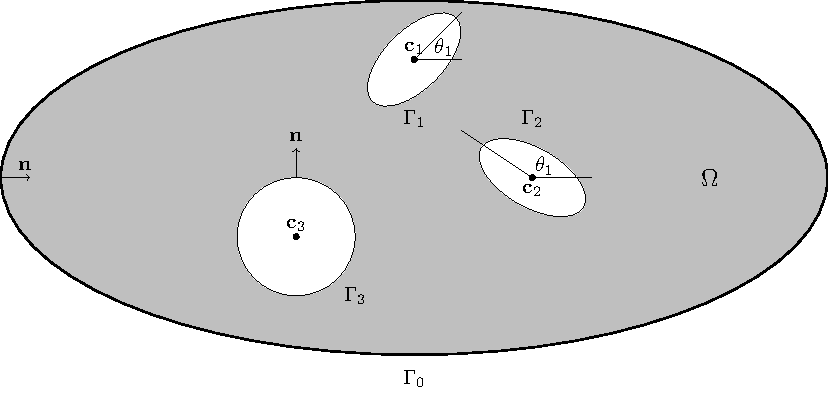
\includegraphics{figures/multiply_connected.pdf}
\caption[Sketch of a multiply connected domain]{Example of a bounded multiply-connected domain. The fluid domain is colored in gray. Obstacles colored in green are mobile bodies and objects colored in red are fixed solid walls.}\label{fig:multiply_connected}
\end{center}
\end{figure}

We now consider a multiply-connected domain consisting of mobile rigid bodies, interior solid walls, and a bounding solid wall.  A sketch of a bounded multiply-connected domain is shown in Figure \ref{fig:multiply_connected}.  Consider a suspension of $n_p$ mobile rigid bodies and $n_w$ interior solid walls. The domain is enclosed by a solid boundary $S_0$.  For each rigid body $V^p_k$, $k=1,\hdots, n_p$, we prescribe the net force and torque $\FF^p_k$ and $L^p_k$, respectively. The translational and rotational velocities of the rigid bodies $\UU_k$ and $\omega_k$ are unknowns. For each solid wall $V^w_\ell$, $\ell=1,\hdots,n_w$, the velocity at any point on its boundary is given, and we solve for the net force and torque $\FF^w_\ell$ and $L^w_\ell$. Each rigid body is bounded by a surface $S^p_k$ and has a center of rotation $\cc^p_k$. The union of all the rigid body surfaces is denoted by $S^p$. Each solid wall is denoted by $S^w_\ell$ and is centered at $\cc^w_\ell$. The union of all the wall surfaces is denoted by $S^w$. 

We represent the velocity as a sum of double-layer potentials around each of the components of the fluid boundary. This results in a nontrivial null space that we address by combining the techniques described for exterior (Section \ref{sec:exterior}) and interior (Section \ref{sec:interior}) problems. The double-layer representation has a single null function from the outer wall (which is not orthogonal to the normal on the outer wall) and $3(n_p+n_w)$ null functions from the rigid bodies and solid walls, those being density functions corresponding to rigid body motions \cite{Ladyzhenskaya1963, Karrila1989, Karrila1991, Power1987}. Therefore for $\xx\in V$ we make the ansatz
\[ \uu(\xx) = \mathcal{D}[\bm{\eta}](\xx) +  \sum\limits_{\ell=1}^{n_w} \left(\Ss[\FF^w_\ell,\cc^w_\ell](\xx) + \RR[L^w_\ell,\cc^w_\ell](\xx)\right)  +  \sum\limits_{k=1}^{n_p} \left(\Ss[\FF^p_k,\cc^p_k](\xx) + \RR[L^p_k,\cc^p_k](\xx)\right),\qquad \xx\in V.\]

The density function $\bm{\eta}$ is defined on the entire surface, i.e. $S_0 \cup S^p \cup S^w$. On the solid walls and the bounding wall, we prescribe a Dirichlet boundary condition, $\uu(\xx) = \mathbf{g}(\xx)$ and on the rigid bodies we prescribe the net force and torque $\FF^p_k$ and $L^p_k$, respectively. Then, the canonical equations for the mobility and resistance problem~\cite{Karrila1989, Karrila1991} are:
\begin{subequations}\label{eq:canonical_velocity}
\begin{equation}\label{eq:canonical_outer}
\begin{aligned}
	-\frac{1}{2}\bm{\eta}(\xx) + \mathcal{D}[\bm{\eta}](\xx) &+ \sum\limits_{\ell=1}^{n_w} \left(\Ss[\FF^w_\ell,\cc^w_\ell](\xx) + \RR[L^w_\ell,\cc^w_\ell](\xx)\right)  + \mathcal{N}_0[\bm{\eta}](\xx) \\&= \mathbf{g}(\xx) -  \sum\limits_{k=1}^{n_p} \left(\Ss[\FF^p_k,\cc^p_k](\xx) + \RR[L^p_k,\cc^p_k](\xx)\right),\qquad \xx\in S_0,
\end{aligned}
\end{equation}
\begin{equation}\label{eq:canonical_wall}
\begin{aligned}
	-\frac{1}{2}\bm{\eta}(\xx) + \mathcal{D}[\bm{\eta}](\xx) &+ \sum\limits_{\ell=1}^{n_w} \left(\Ss[\FF^w_\ell,\cc^w_\ell](\xx) + \RR[L^w_\ell,\cc^w_\ell](\xx)\right)  \\&= \mathbf{g}(\xx) -  \sum\limits_{k=1}^{n_p} \left(\Ss[\FF^p_k,\cc^p_k](\xx) + \RR[L^p_k,\cc^p_k](\xx)\right),\qquad \xx\in S^w, 
\end{aligned}
\end{equation}
\begin{equation}\label{eq:canonical_particle}
\begin{aligned}
	-\frac{1}{2}\bm{\eta}(\xx) + \mathcal{D}[\bm{\eta}](\xx) &+ \sum\limits_{\ell=1}^{n_w} \left(\Ss[\FF^w_\ell,\cc^w_\ell](\xx) + \RR[L^w_\ell,\cc^w_\ell](\xx)\right) - \UU_k - \omega (\xx - \cc^p_k)^\perp \\&=-  \sum\limits_{k=1}^{n_p} \left(\Ss[\FF^p_k,\cc^p_k](\xx) + \RR[L^p_k,\cc^p_k](\xx)\right),\qquad \xx\in S^p.
\end{aligned}
\end{equation}
\end{subequations}
While the left hand side of \eqref{eq:canonical_velocity} has a trivial null space, there are still more unknowns than equations. To close the system, we proceed as in the case of a single rigid body by associating the density function with the net force and torque on each obstacle:
\begin{subequations}\label{eq:canonical_closure}
	\begin{alignat}{3}
		\int_{S^w_\ell} \bm{\eta}~\text{d}S &= \FF^w_\ell, \qquad \int_{S^w_\ell} \bm{\eta}\cdot(\xx - \cc^w_\ell)^\perp~\text{d}S &&= L^w_\ell, &\qquad \ell = 1,\hdots, N_w,\\
		\int_{S^p_k} \bm{\eta}~\text{d}S &= \FF^p_k, \qquad \int_{S^p_k}\bm{\eta}\cdot(\xx - \cc^p_k)^\perp~\text{d}S &&= L^p_k, &\qquad k = 1,\hdots, N_p.\label{eq:particle_closure}
	\end{alignat}
\end{subequations}

Equations \eqref{eq:canonical_velocity} and \eqref{eq:canonical_closure} form an invertible second-kind Fredholm integral equation. They can be solved for the translational and rotational velocities of the rigid bodies and the  net forces and torques on the fixed solid walls. Note that we still require $\int_{S_0\cup S^w} \uu\cdot\nn~\text{d}S = 0$ for global conservation of mass.

Unbounded domains are  treated in a similar manner. In this case, for the disturbance velocity to decay at infinity, the total net force on all the obstacles must be zero. For this reason, we only consider unbounded flow past mobile rigid bodies where we prescribe the net force
\[ \sum\limits_{k=1}^{n_p} \FF^p_k = \mathbf{0}.\]
 The canonical equations in this case become
 \begin{equation}\label{eq:canonical_unbounded}
\begin{aligned}
	-\frac{1}{2}\bm{\eta}(\xx) + \mathcal{D}[\bm{\eta}](\xx) &- \UU_k - \omega(\xx - \cc^p_k)^\perp \\&= -\uu^{\infty} -  \sum\limits_{k=1}^{n_p} \left(\Ss[\FF^p_k](\xx,\cc^p_k) + \RR[L^p_k](\xx,\cc^p_k)\right),\qquad \xx\in S^p_k,\end{aligned}
\end{equation}
along with the closure condition given in \eqref{eq:particle_closure}. 

\subsection{Computing Pressure and Stresses}

We are interested in characterizing rheological properties of the suspension. This requires computing the pressure and stress of the flow. Fortunately, these quantities (and others, such as the vorticity) can be computed as a post-processing step after we have calculated the density function, and the forces and torques on the solid walls and rigid bodies. 

At a point $\xx\in V$, the pressure of the double-layer potential \cite{Quaife2014} is
\begin{equation}\label{eq:dlp_pressure} p^D[\bm{\eta}](\xx) =  \frac{1}{\pi} \int_S \frac{1}{r^2}\left( 1 - 2\frac{\rr\otimes \rr}{r^2}\right) \nn\cdot\bm{\eta}~\text{d}S,\qquad \xx\in V.\end{equation}
At a point $\xx\in V$, the strain rate tensor of the double-layer potential \cite{Quaife2014, Quaife2018} is
\begin{equation}\label{eq:dlp_stress}
\begin{aligned}
	 e^D_{ij}[\bm{\eta}](\xx) = \frac{1}{2\pi}\int_{S} &\frac{1}{r^4}\biggr( r_kn_kr_\ell \eta_\ell\bigg( \delta_{ij} -\frac{8}{r^2}r_i r_j\bigg) \\&+ r_k\eta_k(n_i r_j + n_j r_i) + r_k n_k(\eta_i r_j + r_j \eta_i)\biggr)~\text{d}S, \qquad \xx\in V.
\end{aligned}\end{equation}
We also require the pressure and stresses of the Stokeslets and rotlets,
\begin{equation}\label{eq:stokeslet_pressure}
	p^S(\xx) = \sum\limits_{i=1}^{n_w} \frac{\rr\cdot\FF^w_i}{2\pi r^2} + \sum\limits_{i=1}^{n_p} \frac{\rr\cdot\FF^p_i}{2\pi r^2} \qquad p^R(\xx) = 0, 
\end{equation}
as well as the strain rate of the Stokeslets and rotlets,
\begin{subequations}\label{eq:stokeslet_stress}
\begin{alignat}{2}
	\ee^S(\xx) &= \sum\limits_{i=1}^{n_w} \frac{\rr \cdot\FF^w_i}{4\pi r^2}\left(\mathbf{I} - \frac{2}{r^2}\rr\otimes\rr\right) + \sum\limits_{i=1}^{n_p} \frac{\rr \cdot\FF^p_i}{4\pi r^2}\left(\mathbf{I} - \frac{2}{r^2}\rr\otimes\rr\right), &&\qquad \xx\in V\cup S,\\
	\ee^R(\xx) &= \sum\limits_{i=1}^{n_w}\frac{L^w_i}{r^4}\left(\rr\otimes \rr^\perp + \rr^\perp\otimes\rr\right) + \sum\limits_{i=1}^{n_p}\frac{L^p_i}{r^4}\left(\rr\otimes \rr^\perp + \rr^\perp\otimes\rr\right), &&\qquad \xx\in V\cup S.
\end{alignat}
\end{subequations}
At a point $\xx\in S$, the limiting values of \eqref{eq:dlp_pressure} and \eqref{eq:dlp_stress} must be considered and the resulting surface pressure and strain rate are
\begin{subequations}\label{eq:jump_conditions_stress}
\begin{alignat}{2}
	\ee^D[\bm{\eta}](\xx)_{(i)} &:= + \mathcal{J}[\bm{\eta}](\xx) + \ee^D[\bm{\eta}](\xx),\\
	\ee^D[\bm{\eta}](\xx)_{(e)} &:=  -\mathcal{J}[\bm{\eta}](\xx) + \ee^D[\bm{\eta}](\xx),\\
	p^D[\bm{\eta}](\xx)_{(i)} &:= -\frac{\partial\bm{\eta}}{\partial\bm{\tau}}\cdot\bm{\tau}(\xx) + p^D[\bm{\eta}](\xx),\\
	p^D[\bm{\eta}](\xx)_{(i)} &:= +\frac{\partial\bm{\eta}}{\partial\bm{\tau}}\cdot\bm{\tau}(\xx) + p^D[\bm{\eta}](\xx),
\end{alignat}
\end{subequations}
where
\[ \mathcal{J}[\bm{\eta}](\xx) = \frac{1}{2}\left(\frac{\partial\bm{\eta}}{\partial\bm{\tau}}\cdot\bm{\tau}\right)\begin{pmatrix} 2\tau_x\tau_y & \tau_y^2 - \tau_x^2\\ \tau_y^2 - \tau_x^2 & -2\tau_x\tau_y\end{pmatrix}.\]

Equations \eqref{eq:dlp_pressure}, \eqref{eq:dlp_stress}, \eqref{eq:stokeslet_pressure}, \eqref{eq:stokeslet_stress} along with the jump conditions \eqref{eq:jump_conditions_stress} allow us to compute the strain rate and the pressure at any point $\xx \in V\cup S$. Finally, the pressure and strain rate can be added together to form the total stress. 


 
